% vim: ts=2:sw=2:tw=80:et
\thispagestyle{fancy}
\pagestyle{fancy}
\section{Channel Name}
\section{Specifying Device}

\section{Defining Scaling and Units}
Arbwave allows for non-digital channels to be scaled according to an arbitrary
monotonically decreasing/increasing function.  This allows the user to calibrate
the output of a particular channel for a particular use.  For example, if a
analog voltage output channel is used to change the frequency output of a laser,
it is more convenient for the channel to be calibrated to describe the actual
frequency changes occurring with the laser.

The user can right-click a non-digital channel in the channel menu to access the
scaling dialog.  The scaling dialog, shown in Fig.~\ref{fig:channel:scaling}, gives
access to a table of scaling values that can be used to calibrate the channel.

\begin{figure}[ht]
  \centerline{\includegraphics[width=.8\textwidth]{figures/select-scaling}}
  \caption{Having added some channels, right click an analog channel to
  specify scaling/calibration.}
  \label{fig:channel:select-scaling}
\end{figure}


\begin{figure}[ht]
  \centerline{\includegraphics[width=.5\textwidth]{figures/scaling-v0}}
  \caption{Specify the units and scaling or calibration on analog
  channels.}
  \label{fig:channel:scaling-v0}
\end{figure}


\begin{figure}[hb]
  \centerline{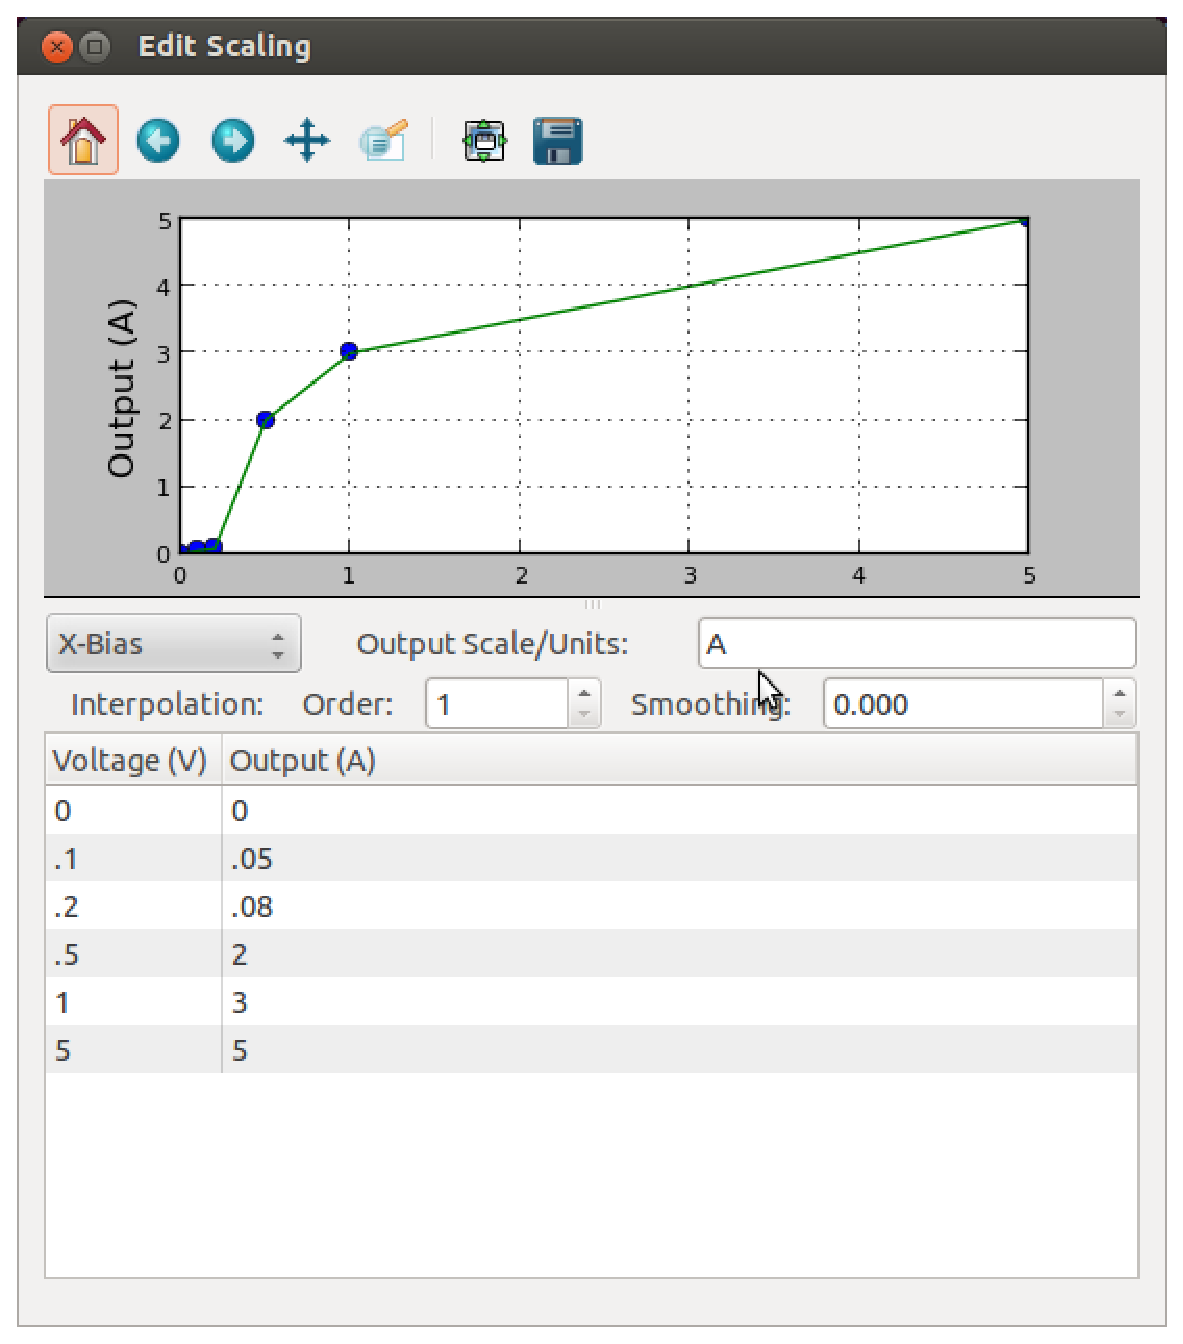
\includegraphics[width=.5\textwidth]{figures/scaling}}
  \caption{
    Using the scaling editor, each channel can be controlled via a set of units
    and scaling that is natural for the experiment.
  }
  \label{fig:channel:scaling}
\end{figure}

Each row of this table consists of a list of voltage settings that produce the
corresponding list of output values (such as laser frequency).  The list in each
column of each row may include one or more items although it is critical that
the two cells of a row must contain the same number of elements.

In addition to simple scaling, as shown in Fig.~\ref{fig:channel:scaling}, it is
also possible to apply a $n^{\rm th}$-order smoothing function to the data.
This may be helpful if the calibration data is somewhat noisy.

\section{Static Values}
\section{Enabling}
